As mentioned before, the main goal of the overall project is to develop method not requiring the interference of the human at any stage and thus being fully objective, which is contrary with previously described steps. In target method, the steps descried in sections \ref{subsec:labelling} - \ref{subsec:pelvis} will be replaced by deep learning techniques. The designed neural networks should not require registration of the images, which is usually the most inconvenient step. Not only is it very time-consuming (motion correction of the one time series used in the project lasts \textasciitilde 6h) but also it causes loss of information. As a~result, the method will enable fast and efficient automated GFR estimation directly from the DCE-MRI without any previous preprocessing.
Although applying deep learning is still under intensive development, current studies already have showed promising results. What was achieved so far, is segmentation of the both left and right kidney from raw DCE-MRI images using convolutional neural network. 

Convolutional Neural Networks (CNN) were inspired by the architecture of the animal visual cortex and are specifically suitable for image recognition. It was shown that numerous neurons in the visual cortex are sensitive only to the stimuli located in the small limited region of the visual field. In short terms, these neurons have small local receptive fields, which can overlap and all together cover whole visual field. What is more, certain neurons are activated only by horizontal lines, whereas the others reacts to these of different orientations.
Furtermore, some neurons with bigger receptive fields responds to the more complex patterns being the assembly of the lower-level patterns, which leads to the conclusion that the higher-level neurons are based on the outputs of neighbouring lower-level neurons \cite{hubel1968receptive,handson}.  The described complex system composed of the neurons ordered in a columnar fashion is able to detect all kinds of patterns in whole visual field creating the visual perception. The above idea is shown on Figure \ref{fig:visual_cortex}. 
 

\begin{figure*}
	\centering
	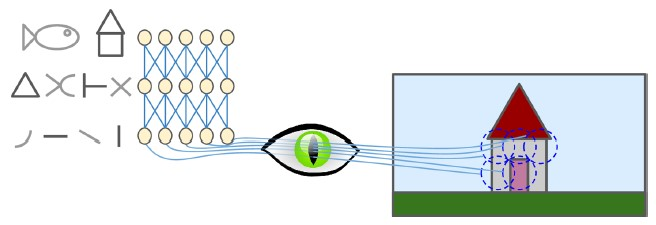
\includegraphics[width = \linewidth]{img/visual_cortex}
	\caption{Local receptive fields in the visual cortex \cite{handson}.}
	\label{fig:visual_cortex}
\end{figure*}

From the finding of the studies on visual cortex convolutional neural networks emerged. Unlike the traditional neural networks, their architecture incorporates multiple convolutional layers, neurons of which  connect to the subregions of the previous layers instead of being fully-connected. The neurons are not sensitive to the areas outside of these subregions in the image.
Each of the layer learn to recognise different feature. The deeper the layer is, the more detailed 

The network has a dual pathway architecture incorporating both local and global information in the volumes. It consist of \color{red}(?) \color{black} layers.
The idea of transfer learning was applied. 

\begin{figure*}
	\centering
	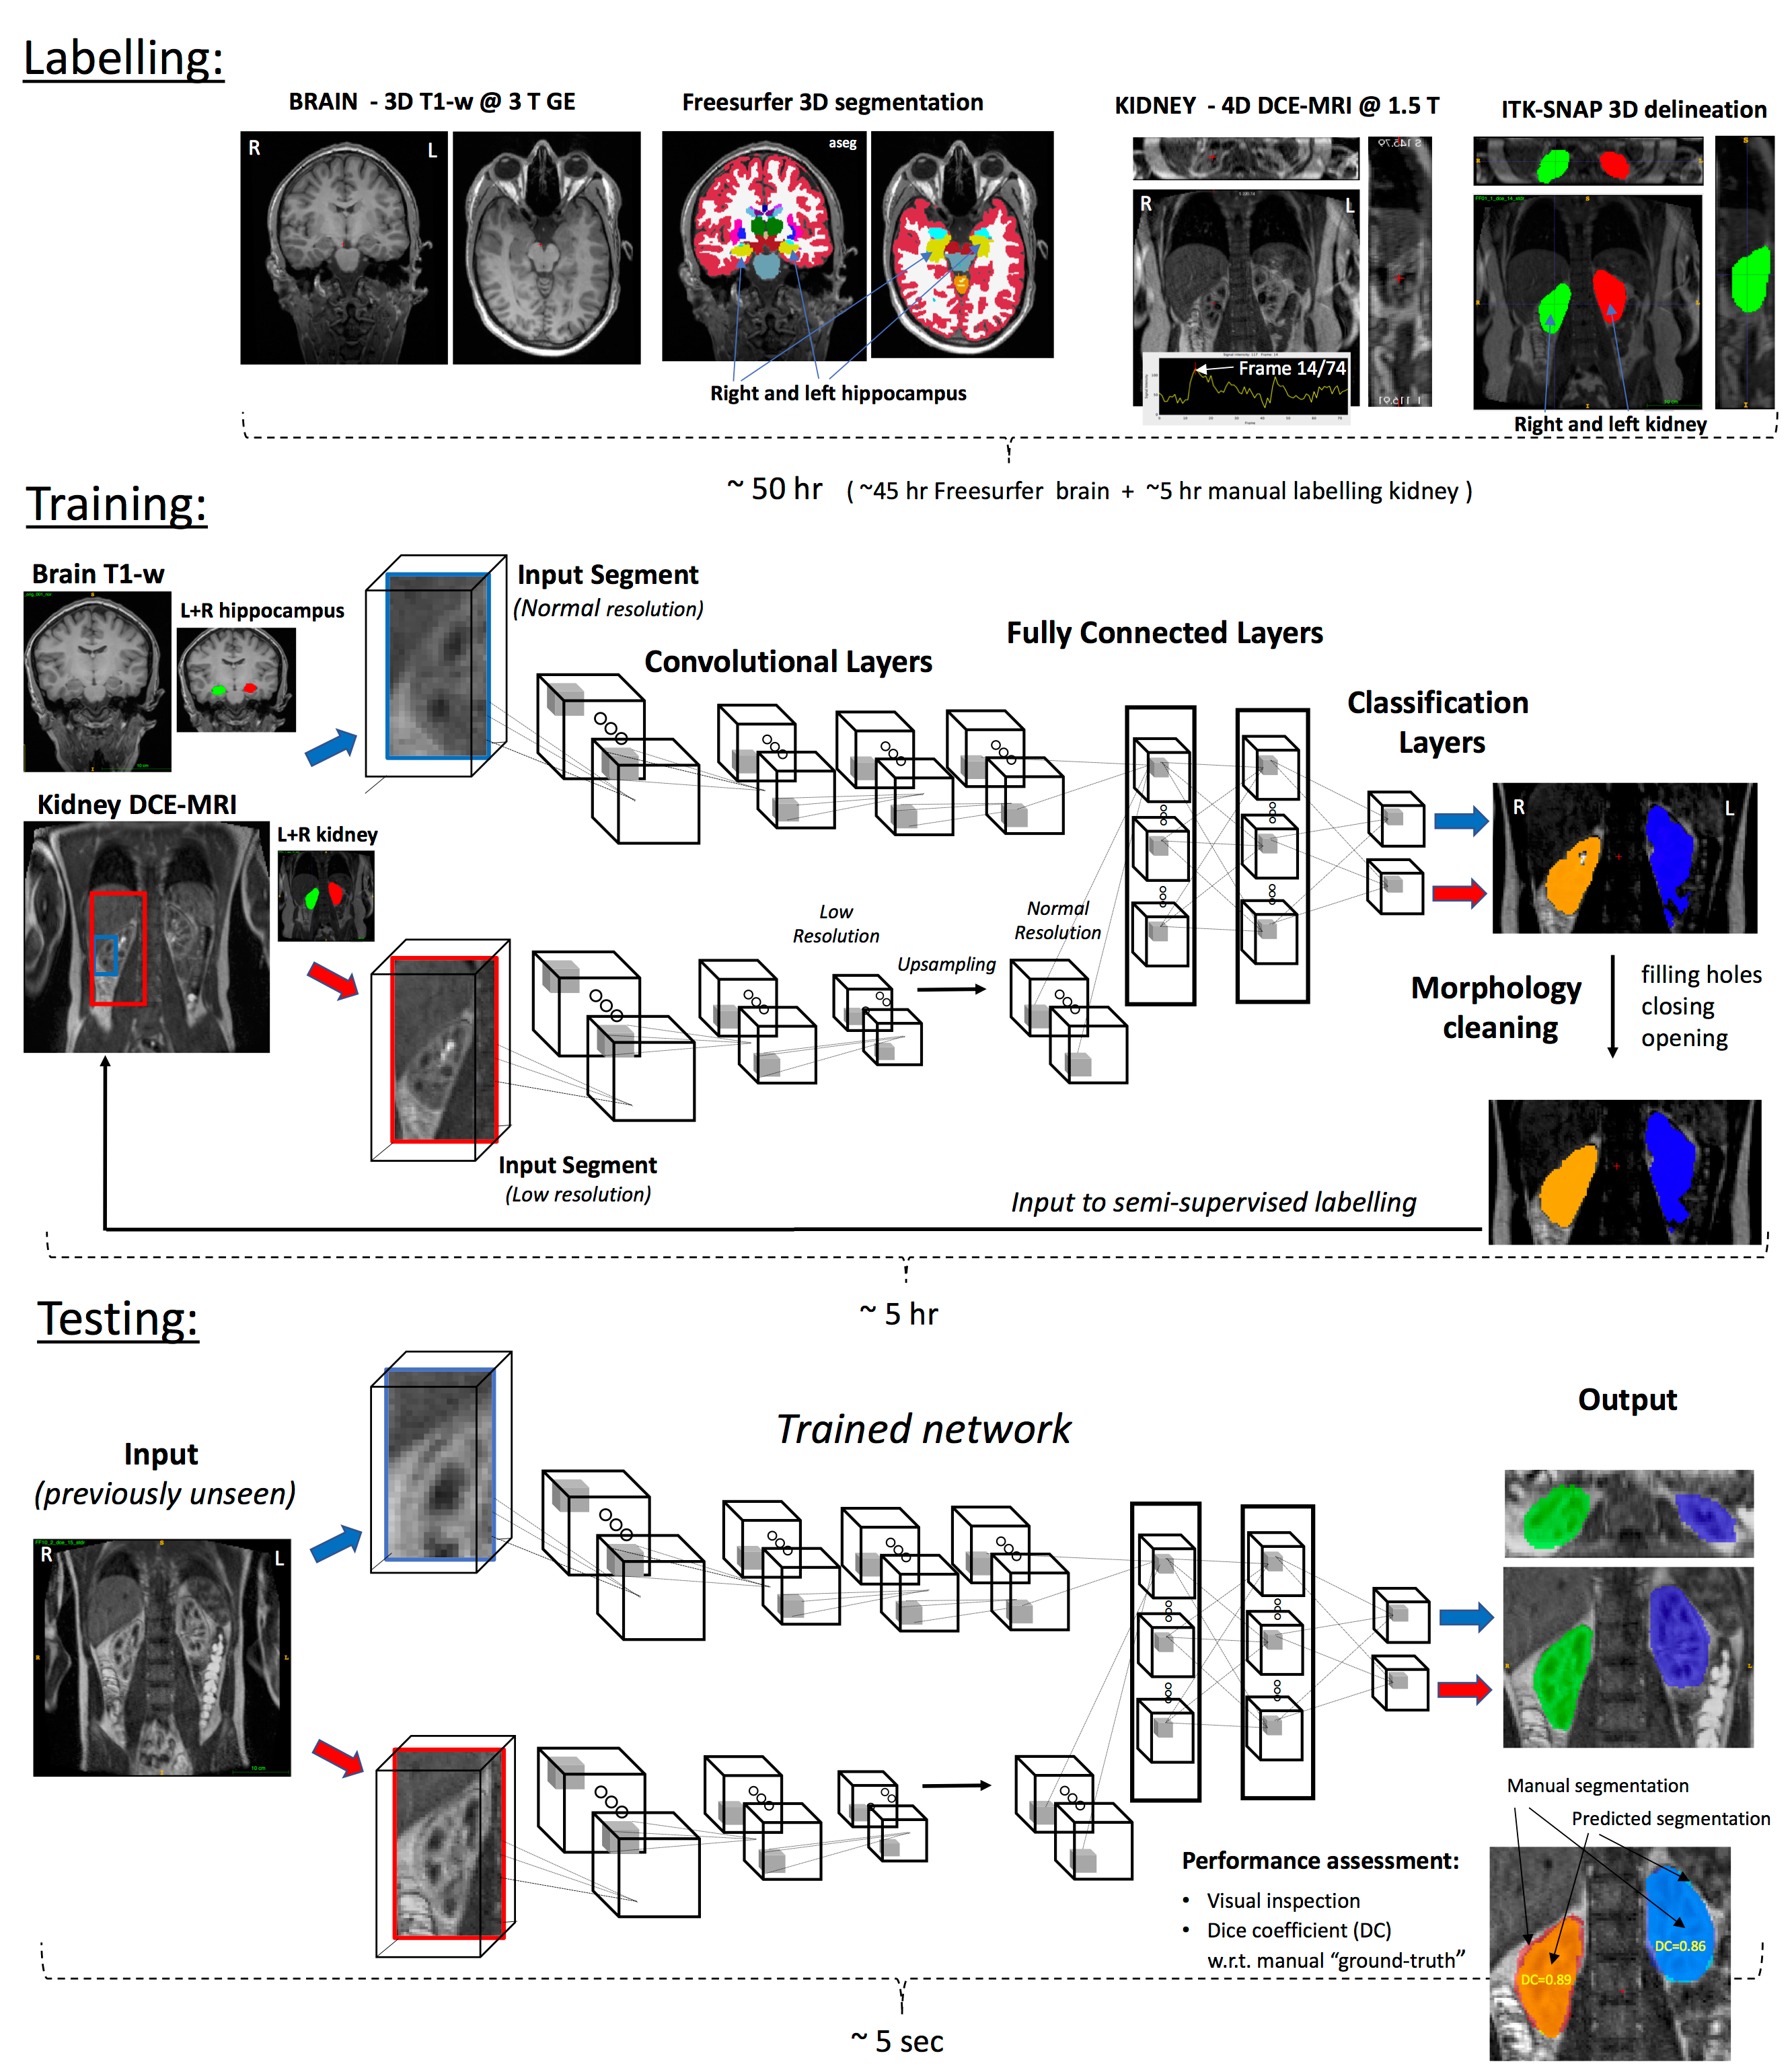
\includegraphics[width = \linewidth]{img/cnn}
	\caption{}
	\label{fig:cnn}
\end{figure*}

